\chapter{DESENVOLVIMENTO DA SOLUÇÃO}
\thispagestyle{myheadings}

Os resultados e discussões apresentados a seguir referem-se aos experimentos realizados durante 
a reestruturação dos processos de ETL do BDMalhas. As análises baseiam-se nas métricas definidas 
na metodologia, permitindo comparar o desempenho da arquitetura proposta com a solução legada 
baseada em SSIS.

\section{Arquitetura proposta para a reestruturação da plataforma de dados}

A seguir, apresenta-se o sistema de ETL desenvolvido para materializar a proposta de 
reestruturação da plataforma de dados da SEFAZ-PB, utilizando como referência o sistema BDMalhas.
A solução contempla tanto a reestruturação das pipelines de ETL quanto a adoção 
de uma nova arquitetura visando atender às demandas de processamento e análise de grandes 
volumes de dados. Também são apresentados os principais aspectos da implementação da solução.

\section{Arquitetura do BDMalhas}

O BDMalhas é um projeto composto por sistemas integrados que auxiliam o processo de 
fiscalização tributária da SEFAZ-PB por meio da análise de documentos fiscais, como NFe, 
NFCe e EFD. Nesse cenário, os dados oriundos do Sistema de Administração Tributária e 
Financeira (ATF), que atua como \textit{System of Record} (SOR), ou seja, o sistema considerado fonte 
oficial e autorizada das informações tributárias e financeiras da Secretaria. Essas informações 
são coletadas por meio de um processo de ETL implementado em SSIS, e em seguida, armazenados 
em uma área \textit{staging} (área de preparação dos dados). 

Em seguida, a área de \textit{staging} é utilizada para a geração de bases de dados analíticas no 
formato de malhas fiscais, a serem acessadas pelos auditores para atividades de análise através 
do Sistema de Controle e Análise das Malhas Fiscais (SCAMF).

\begin{figure*}[ht!]
    \centering
    \caption{Visao Geral da Arquitetura Antiga do BDmalhas}\label{fig:arq_ant_bdmalha}
    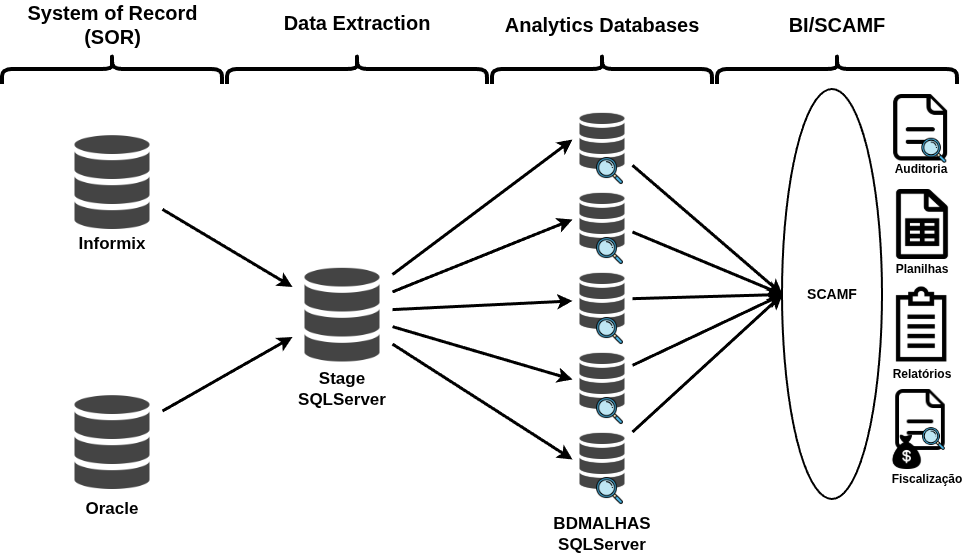
\includegraphics[width=0.8\textwidth]{imagens/ArquiteturaAntiga_bdmalhas}\\
    {\small Fonte: Elaborado pelo autor, 2026}
\end{figure*}

Nesse sentido, a Figura \ref{fig:arq_ant_bdmalha} apresenta a arquitetura de dados do BDMalhas, estruturada nas seguintes 
camadas:

\begin{itemize}
    \item \textbf{System of Record (SOR):} camada responsável pela origem dos dados. Nela encontram-se os 
    bancos de dados transacionais do sistema ATF, implementados nas plataformas Informix e Oracle.

    \item \textbf{Data Extraction:} camada responsável pela extração dos dados. Por meio de processos de 
    ETL (Extract, Transform and Load), os dados são extraídos do SOR, submetidos às transformações 
    necessárias e carregados em uma área intermediária de armazenamento.

    \item \textbf{Analytical Databases:} camada responsável pela consolidação e disponibilização analítica 
    das informações. A partir dos dados armazenados na área de staging, são executados processos 
    de transformação e enriquecimento que resultam na construção de bases analíticas e malhas 
    fiscais destinadas ao consumo pelo SCAMF.

    \item \textbf{BI/SCAMF:} camada de apresentação e consumo das informações. Nessa camada, os dados 
    são disponibilizados aos fiscais e contribuintes por meio do sistema SCAMF, responsável por 
    fornecer recursos de consulta, visualização e análise das informações produzidas pelas camadas 
    anteriores.
\end{itemize}

\section{Arquitetura Reestruturada do BDMalhas}

A nova arquitetura implementada para o BDMalhas incorpora um Data Lake, desenvolvido pela 
Universidade Federal da Paraíba (UFPB) em parceria com a SEFAZ-PB, como principal fonte de 
dados para a etapa de extração. O Data Lake consiste em um repositório centralizado que atua 
no armazenamento e integração de grandes volumes de dados provenientes das diferentes fontes 
da secretaria.

Dessa forma, os processos passam a extrair informações de um ambiente estruturado para cenários 
de Big Data, simplificando as consultas e aumentando a eficiência das etapas de integração e 
processamento dos dados.

Ademais, houve a substituição do SQL Server Integration Services (SSIS) pelo Apache Airflow como 
plataforma de orquestração dos pipelines de dados, juntamente com a adoção do Apache Spark como 
mecanismo de processamento distribuído. Essa mudança  visa proporcionar maior escalabilidade, 
flexibilidade e capacidade de processamento.

Por fim, o banco de dados da camada de staging foi substituído por um banco de dados colunar, 
mais adequado a cenários de Big Data. Esse modelo de armazenamento proporciona maior eficiência 
no processamento de grandes volumes de dados e melhor desempenho em consultas analíticas, 
características essenciais para a nova arquitetura proposta.

\begin{figure*}[ht!]
    \centering
    \caption{Visao Geral da Arquitetura Nova do BDmalhas}\label{fig:arq_nova_bdmalha}
    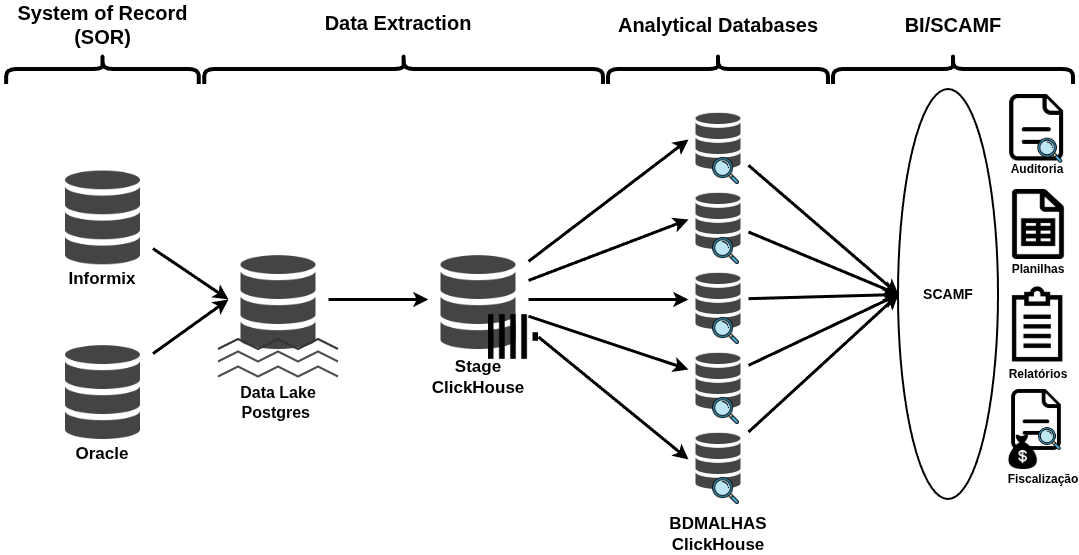
\includegraphics[width=0.8\textwidth]{imagens/ArquiteturaNova_bdmalhas}\\
    {\small Fonte: Elaborado pelo autor, 2026}
\end{figure*}

A Figura \ref{fig:arq_nova_bdmalha} apresenta a nova arquitetura de dados do BDMalhas, com alterações para as 
seguintes camadas:

\begin{itemize}
    \item \textbf{Data Extraction:} passa a ter mais uma camada, um Data Lake implementado em 
    Postgres e gerido pela UFPB, de onde os dados são extraídos, alimentado a base de staging.

    \item \textbf{Analytical Databases:} no \textit{staging}, são executados processos de transformação e 
    enriquecimento que resultam na construção de bases analíticas e malhas fiscais destinadas
    ao consumo pelo SCAMF.
\end{itemize}

Dado o contexto da nova stack tecnológica adotada na reestruturação, o processo de ETL 
inicia-se com a extração dos dados a partir do Data Lake PostgreSQL da SEFAZ-PB. 
O Apache Airflow é responsável pela orquestração dos fluxos de execução, estruturados em 
DAGs (Directed Acyclic Graphs) compostas por tasks executadas de forma sequencial ou 
paralela, mantendo a mesma lógica operacional anteriormente implementada em Microsoft SSIS.

Contudo, diferentemente da arquitetura anterior, o Airflow não realiza diretamente o 
processamento das cargas de dados, atuando apenas como mecanismo de orquestração. 
As operações de transformação e carga de dados são delegadas a um \textit{cluster} Spark composto 
por múltiplos nós computacionais, responsável pelo processamento distribuído dos dados e 
posterior inserção no ambiente de \textit{staging}.

\section{Benefícios e considerações Arquiteturais}

A adoção de Airflow é justificada por proporcionar um ambiente mais flexível e 
desacoplado para construção e manutenção dos pipelines de ETL, permitindo que os 
fluxos sejam desenvolvidos de forma programática, diferentemente da abordagem utilizada 
pelo SSIS. Além disso, a ferramenta disponibiliza aos administradores recursos nativos de 
monitoramento das execuções, rastreamento de falhas e gerenciamento operacional dos 
pipelines, contribuindo para maior controle e confiabilidade do processo.

Junto a isso, destaca-se a adoção do Apache Spark como mecanismo de processamento 
distribuído, com o objetivo de viabilizar o processamento eficiente dos dados em tempo 
hábil, além de permitir escalabilidade horizontal conforme o aumento da demanda 
computacional. Essa abordagem atende diretamente às necessidades dos fiscais, que 
dependem do acesso rápido e confiável às informações processadas para execução de suas 
atividades de fiscalização.

Dessa forma, a combinação entre Airflow e Spark permite construir uma arquitetura mais 
robusta, escalável e aderente às demandas operacionais e estratégicas da secretaria e do 
sistema BDMalhas.

Em síntese, a arquitetura proposta consolida a reestruturação da plataforma de dados do 
BDMalhas por meio da adoção de tecnologias voltadas ao processamento distribuído e à 
orquestração de pipelines, estabelecendo uma base mais escalável e flexível para os 
processos de ETL. Na sequência, é apresentada uma avaliação dos resultados obtidos com essa 
reestruturação, por meio da comparação entre o sistema original e o sistema desenvolvido.